\documentclass{beamer}
\usepackage[utf8]{inputenc}

\usetheme{Madrid}
\usecolortheme{default}
\useinnertheme{circles}

\definecolor{Logo1}{rgb}{0.208, 0.2865, 0.373}
\definecolor{Logo2}{rgb}{0.000, 0.674, 0.863}

\setbeamercolor*{palette primary}{bg=Logo1, fg=white}
\setbeamercolor*{palette secondary}{bg=Logo2, fg=white}
\setbeamercolor*{palette tertiary}{bg=white, fg=Logo1}
\setbeamercolor*{palette quaternary}{bg=Logo1,fg=white}
\setbeamercolor{structure}{fg=Logo1} % itemize, enumerate, etc
\setbeamercolor{section in toc}{fg=Logo1} % TOC sections

\usepackage{graphicx,animate}
%------------------------------------------------------------
%This block of code defines the information to appear in the
%Title page
\title[Linear Algebra] %optional
{Orthogonality, and Something Interesting...}

\subtitle{Lecture 7}

\author[11910803@mail.sustech.edu.cn] % (optional)
{
    Zhang Ce
}

\institute[] % (optional)
{
    Department of Electrical and Electronic Engineering\\
    Southern University of Science and Technology
}

\date[2021.11.9] % (optional)
{2021.11.9}


%End of title page configuration block
%------------------------------------------------------------



%------------------------------------------------------------
%The next block of commands puts the table of contents at the
%beginning of each section and highlights the current section:

\AtBeginSection[]
{
\begin{frame}
    \frametitle{Table of Contents}
    \tableofcontents[currentsection]
\end{frame}
}
%------------------------------------------------------------


\begin{document}

%The next statement creates the title page.
\frame{\titlepage}


%---------------------------------------------------------
%This block of code is for the table of contents after
%the title page
\begin{frame}
\frametitle{Table of Contents}
\tableofcontents
\end{frame}
%---------------------------------------------------------
\section{Orthogonal Vectors and Subspaces}
\begin{frame}{Inner Product (Dot Product)}
Actually, you have learnt that in your senior high school...

\vspace{3pt}
If I give you 2 vectors $\left[ \begin{array}{c}
	1\\
	2\\
\end{array} \right] ,\left[ \begin{array}{c}
	3\\
	1\\
\end{array} \right]$, how to compute its inner products?

\begin{equation*}
    \left[ \begin{array}{c}
        1\\
        2\\
    \end{array} \right] \cdot \left[ \begin{array}{c}
        3\\
        1\\
    \end{array} \right] =1\times 3+2\times 1=5
\end{equation*}

Recall matrix multiplications, which rule for matrix multiplication is similar to this?

\begin{equation*}
    \left[ \begin{matrix}
        1&		2\\
    \end{matrix} \right] \left[ \begin{array}{c}
        3\\
        1\\
    \end{array} \right] =3+2=5
\end{equation*}

Therefore, for 2 vectors $u$ and $v$, the inner product is $u^Tv$.

\vspace{3pt}
Take a deeper look, the result $5$ shows us... Think in geometrical way!
\end{frame}

\begin{frame}{Inner Product (Dot Product)}
\begin{figure}
    \centering
    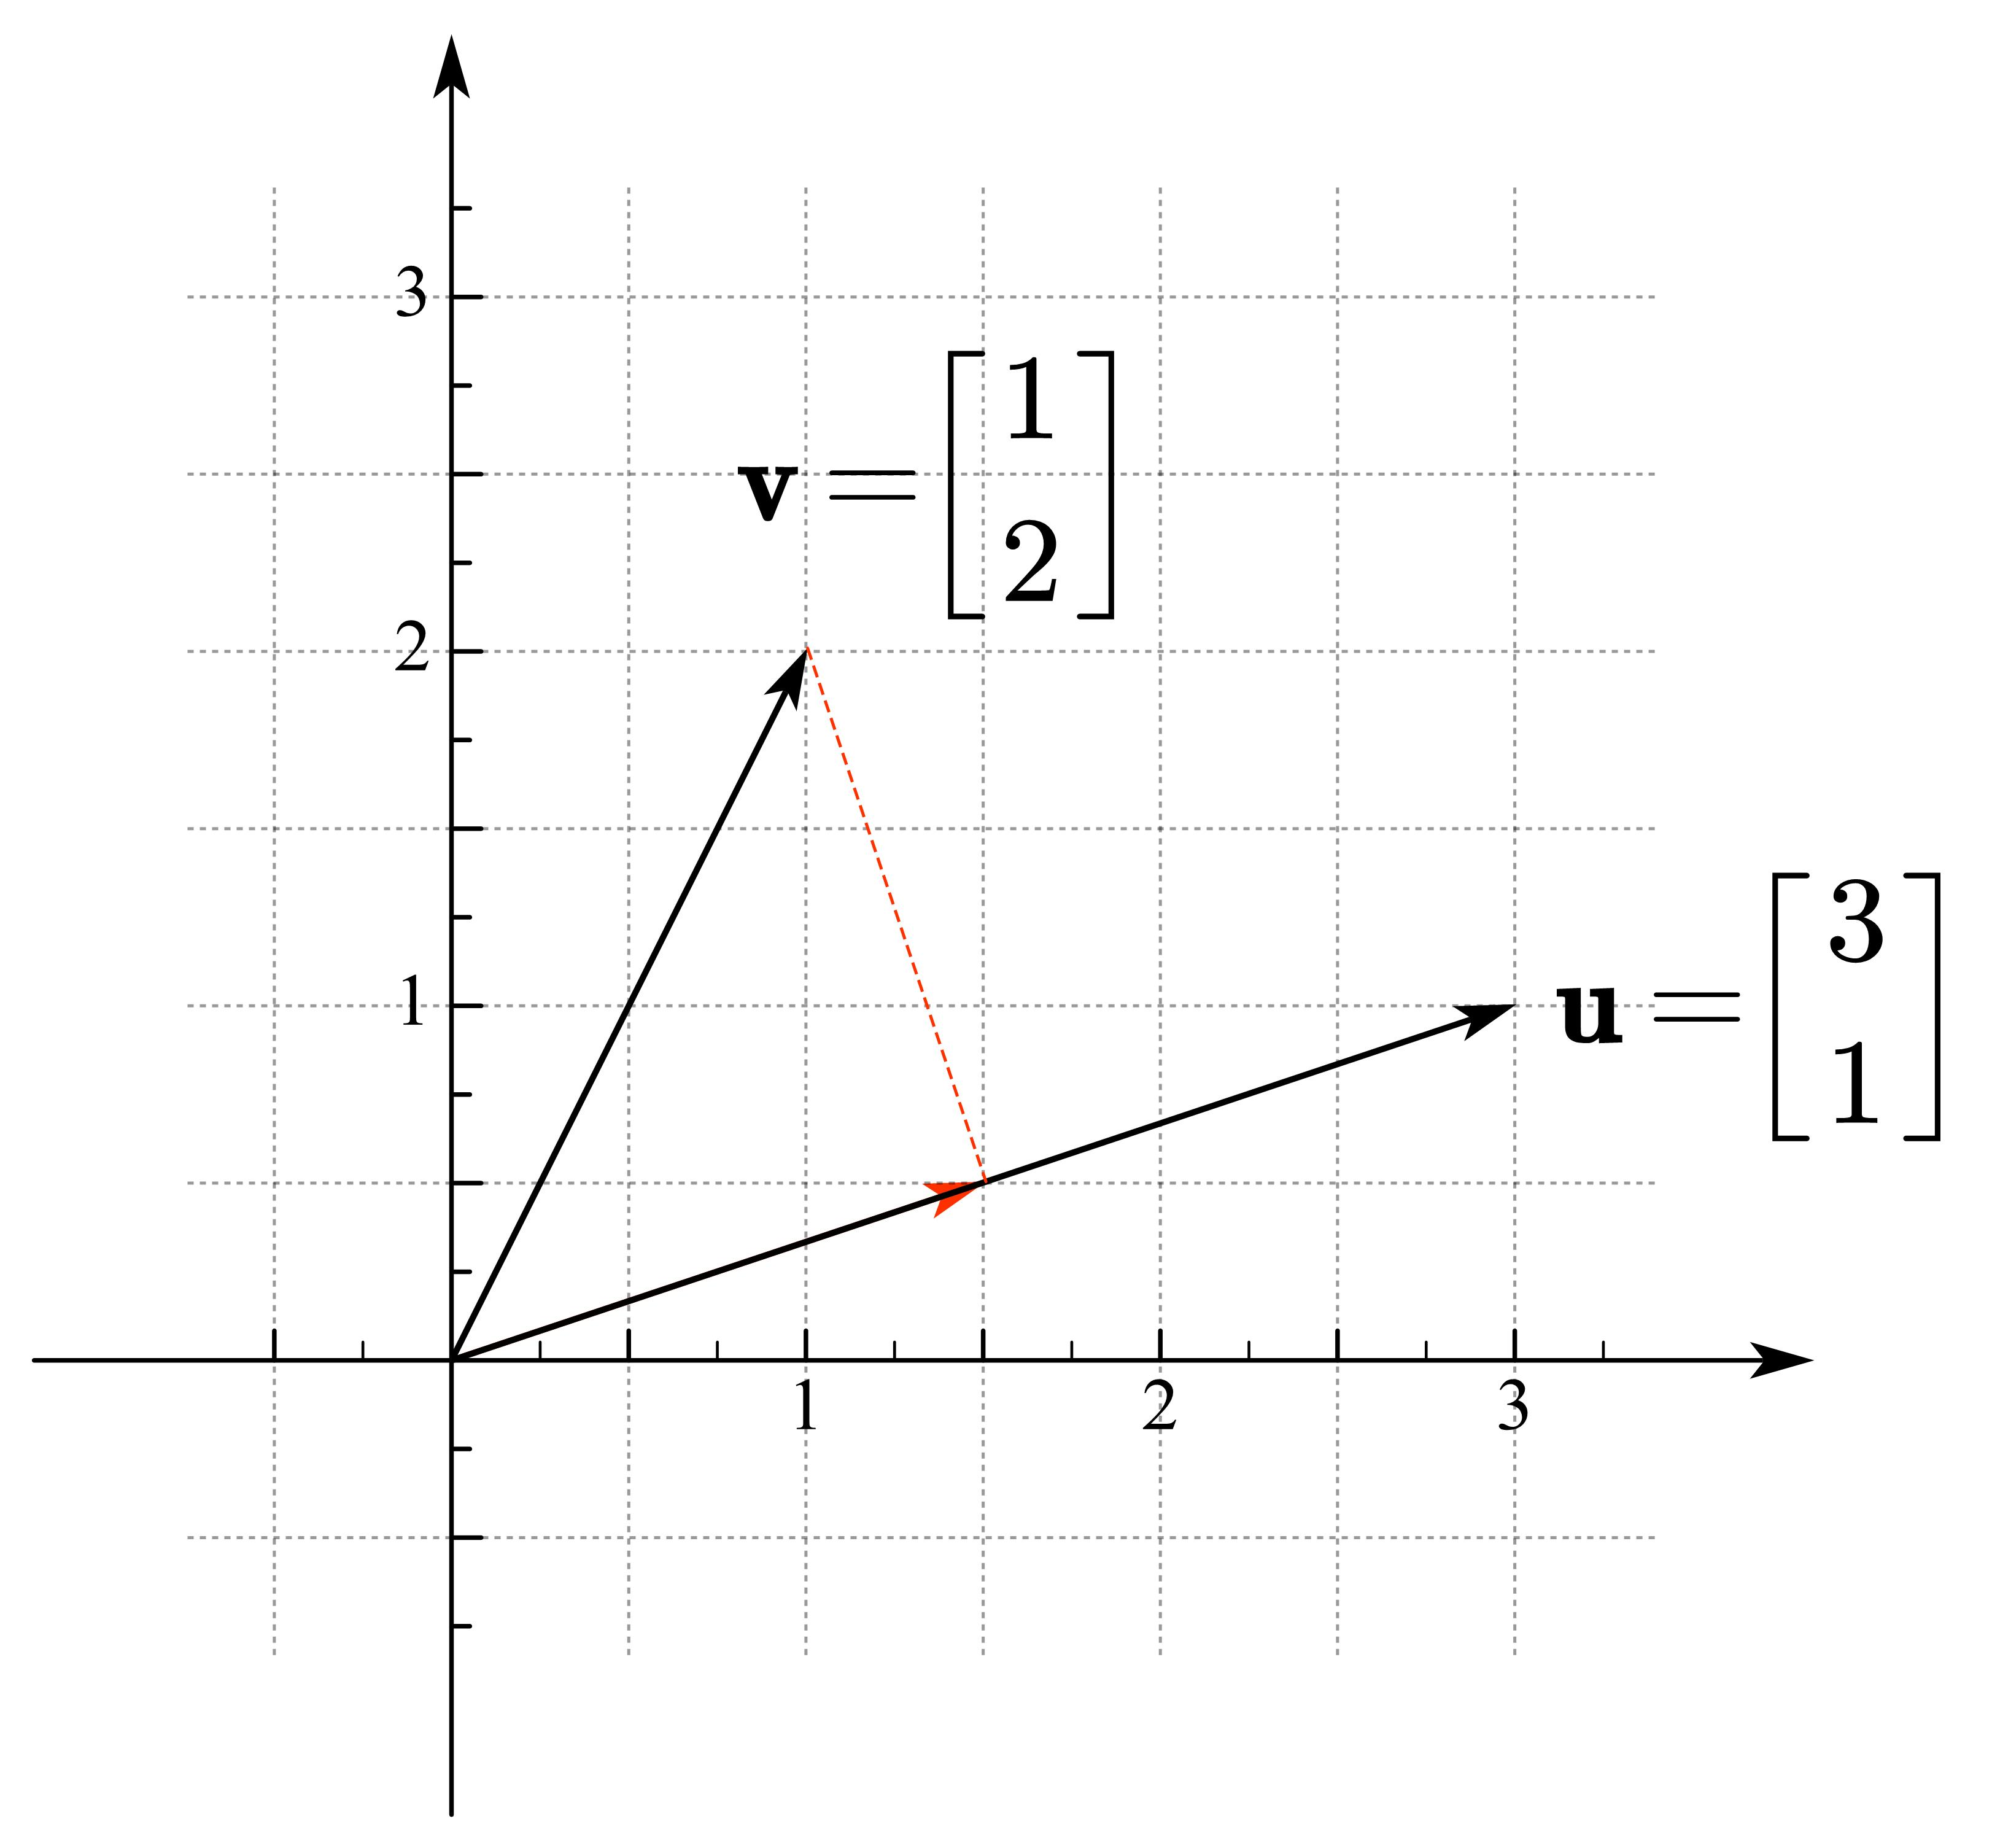
\includegraphics[width=0.47\textwidth]{ip.jpg}
\end{figure}

In my perspective, there inner product reflects their relevance. If the inner product can take the maximum or minimum value, then the vectors are dependent. While if the inner product is greater than zero, they point to the same direction, if it equals to zero, they have nothing to do with each other (perpendicular).
\end{frame}

\begin{frame}{Orthogonal Vectors and Subspaces}
Which value of inner product can let you realize that the vectors are perpendicular (\alert{orthogonal})?
\begin{equation*}
    u^Tv=0
\end{equation*}

Then we can further extend this definition to subspaces, if all the vectors in subspace $A$ are orthogonal to all the vectors in subspace $B$, then suspaces $A$ and $B$ are orthogonal.

\vspace{3pt}
One good question to ask: Is the blackboard plane perpendicular to the ground? But are they orthogonal?

\vspace{3pt}
Well, two orthogonal subspaces can only have the origin in common, and that is from the restriction of subspaces!
\end{frame}

\begin{frame}{Projections}
Let's start from geometrical view.
\begin{figure}
    \centering
    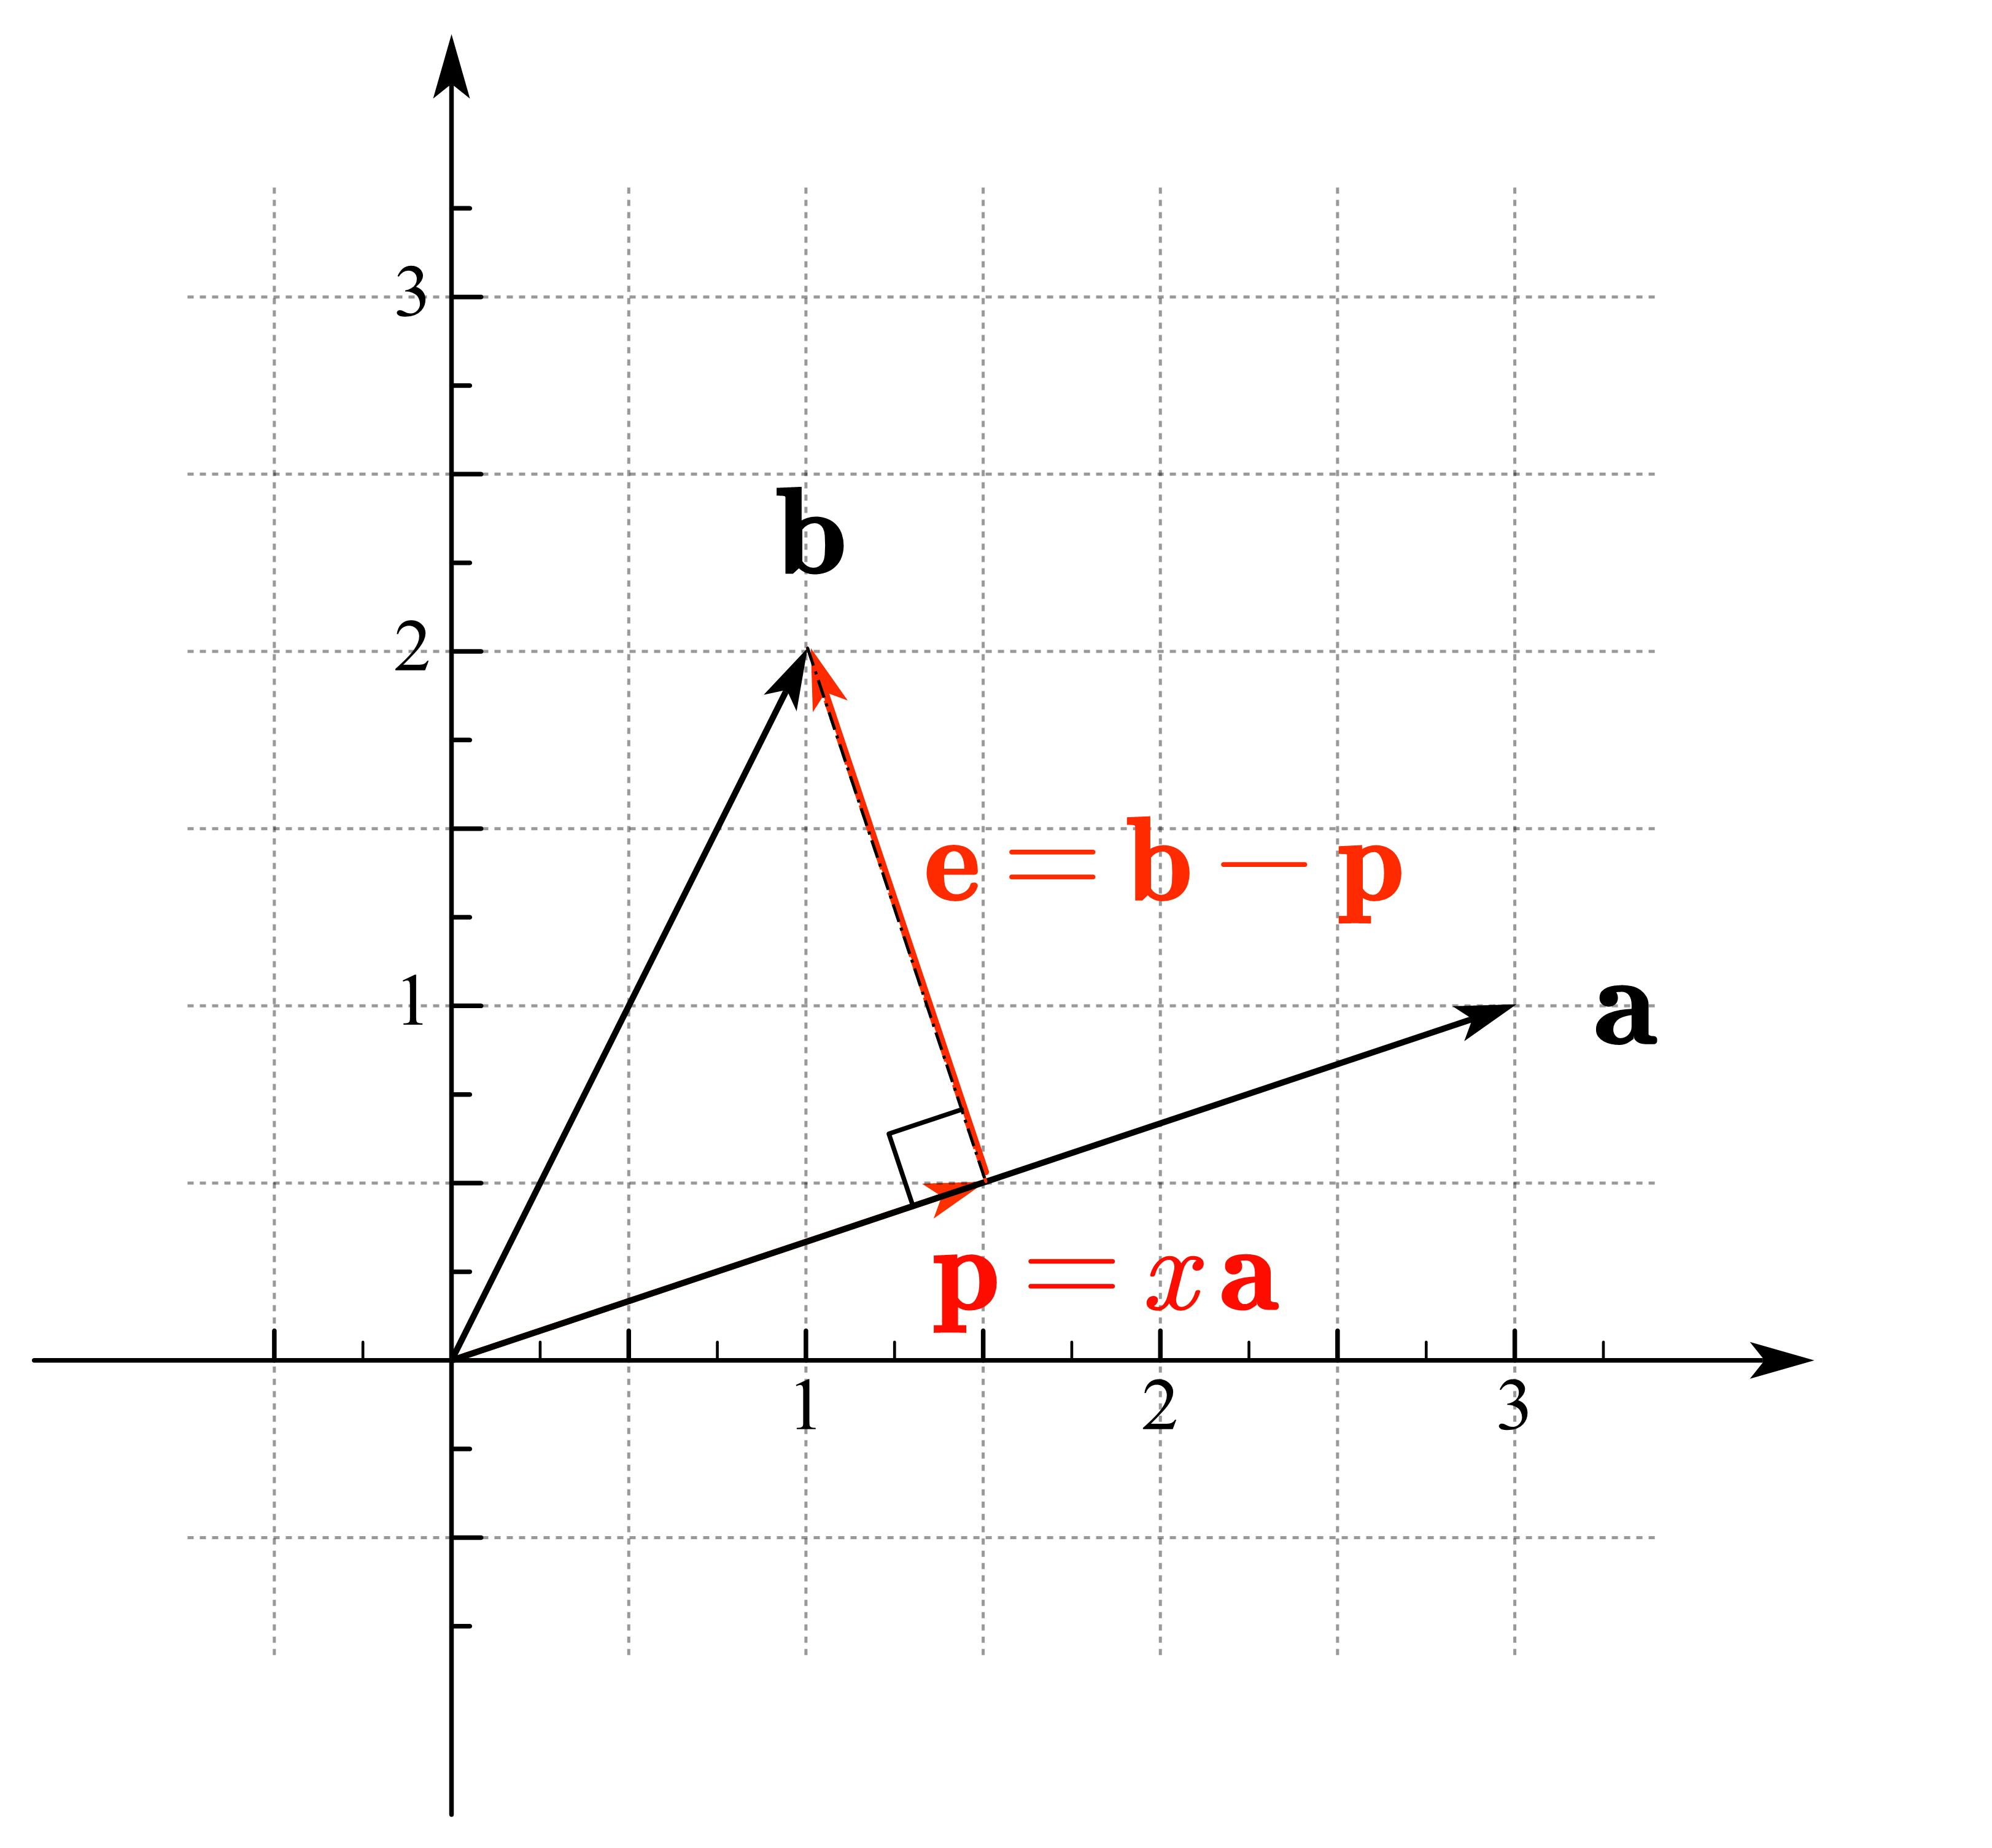
\includegraphics[width=0.47\textwidth]{projection.jpg}
\end{figure}
\end{frame}
\end{document}